\problemWithTimeMem{罗马斗兽场}{1 second}{1024MB}

在一个圆形斗兽场的围墙上均匀插着$n$根木桩,按顺时针顺序编号为$1$,$2$,$3$,$\cdots$,$n$($n$号木桩与$1$号木桩相邻)。

scutsky和byyq将进行一个游戏,byyq可以进行若干次操作,每次操作可以用绳子连接两根不同的木桩$i,j$($1\leqslant i,j\leqslant n$)。要注意的是,byyq连接的绳子不能在非木桩处相交,并且连接$i$,$j$的绳子最多只能有一根。

按照约定,scutsky将从$1$号木桩出发,在不能跨过或钻过绳子并且不离开斗兽场并且不越过木桩的情况下,从任意方向出发,设法到达目标木桩,而byyq则要阻止他。现在scutsky和byyq想知道,当目标木桩分别是$1$,$2$,$3$,$\cdots$,$n$号木桩时,byyq有多少种方案阻止scutsky。两种方案被视为不同当且仅当在一种方案存在$i$,$j$($1\leqslant i,j\leqslant n$)被连接了而另一种方案没有。\textbf{注意:连接$i$,$j$和连接$j$,$i$没有区别。}

本题将会给你多个测试样例,在每个测试样例中,你需要输出$n$个整数,第$i$个整数表示byyq有多少种方案使得scutsky不能从$1$号木桩走到$i$号木桩,结果对$998244353$取模。

\mysec{Input}

第一行包含一个整数 $T$($1\leqslant T \leqslant 1000$),表示测试数据的组数。

每组测试数据输入一个整数 $n$($1 \leqslant n \leqslant 5000$)。

数据保证$\sum n\leqslant 1000000$。

\mysec{Output}

对于每组测试数据,每行输出$n$个整数,第$i$个整数表示byyq有多少种方案使得scutsky不能从$1$号木桩走到$i$号木桩,结果对$998244353$取模。

\ACMIO{Sample 1}{%
4

3

4

5

7
}{%
0 0 0 

0 0 16 0 

0 0 160 160 0 

0 0 13696 16768 16768 13696 0 
}

\mysec{Hint}

$n=4$,$i=3$的所有情况:

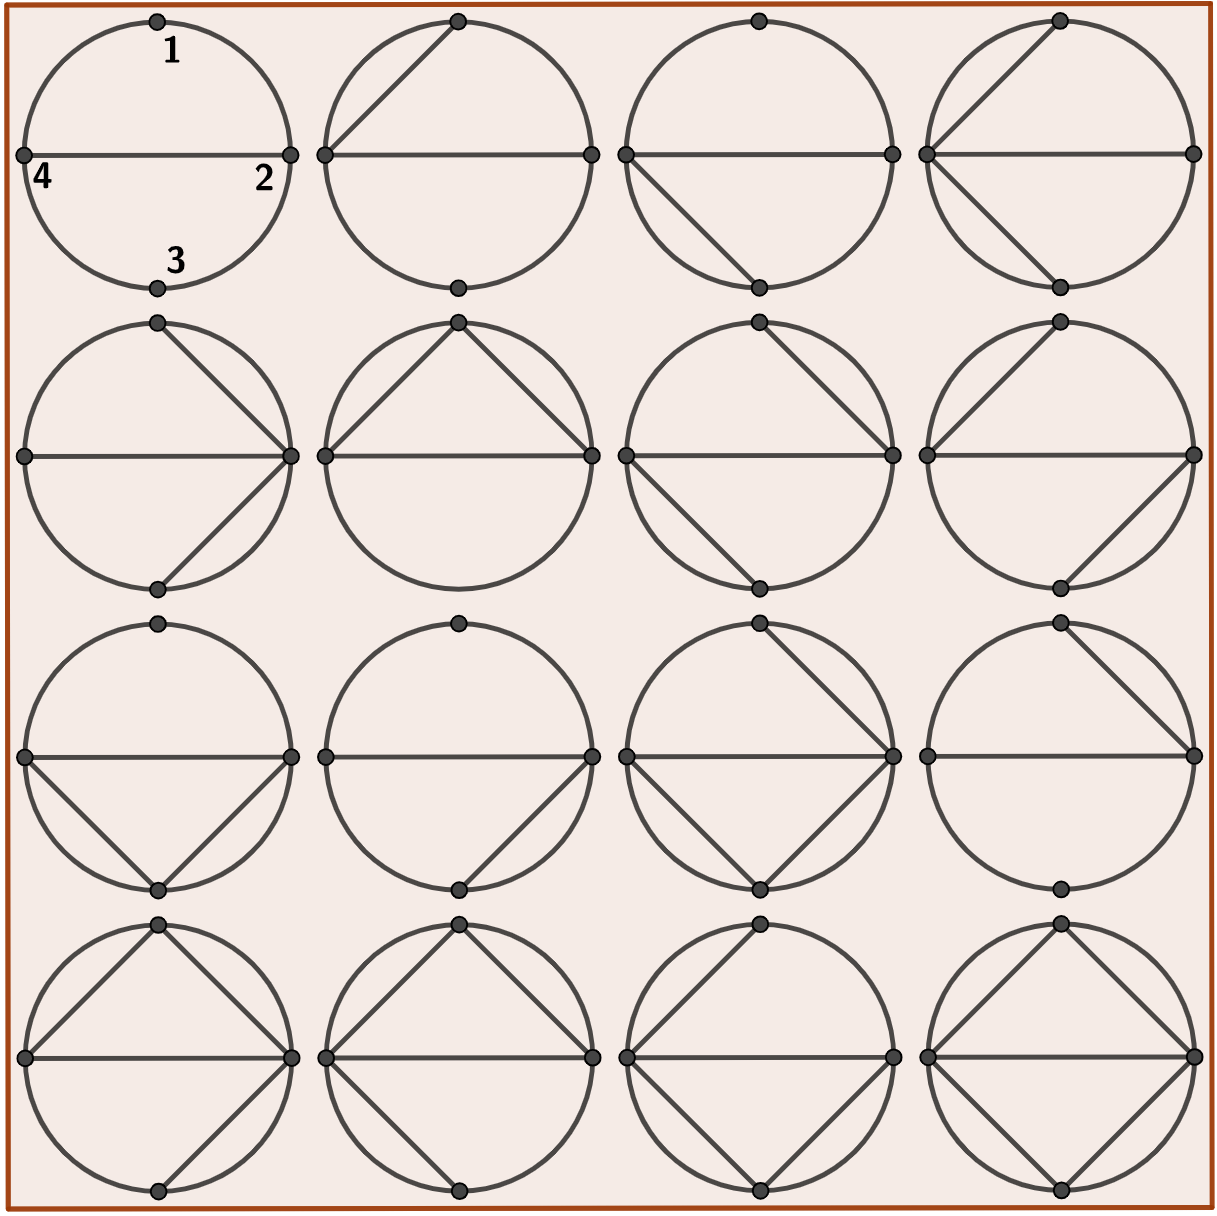
\includegraphics[width=.5\linewidth]{image2.png}